%versi 2 (8-10-2016) 
\chapter{Pendahuluan}
\label{chap:intro}
   
\section{Latar Belakang}
\label{sec:label}

Sekitar tahun 2015, perusahaan PT DNArtworks Komunikasi Visual membuat aplikasi Rugby Indonesia yang memanfaatkan Apache Cordova. Aplikasi tersebut memiliki: 
\begin{itemize}
    \item Halaman \textit{Latest News} yang diambil dari \url{https://rugbyindonesia.or.id} dengan~memanfaatkan~protokol~RSS.
    \item Halaman \textit{Fixture \& Results} yang diambil dari \url{https://rugbyindonesia.or.id}.
    \item Halaman \textit{Teammate Photos} dengan fungsi:
    \begin{itemize}
        \item Pengguna dapat langsung mengambil foto dari aplikasi tersebut.
        \item Pengguna dapat langsung memberikan \textit{frame} terhadap foto tersebut.
        \item Pengguna dapat langsung menggunggah foto tersebut ke dalam galeri publik.
    \end{itemize}
    \item Halaman \textit{Rugby Clubs} yang memiliki fungsi di mana pengguna dapat langsung mendaftar ke dalam \textit{Rugby Clubs} yang berada di Indonesia.
    \item Fungsi \textit{Push Notifications}.
\end{itemize}

\begin{figure} [!h]
    \centering
    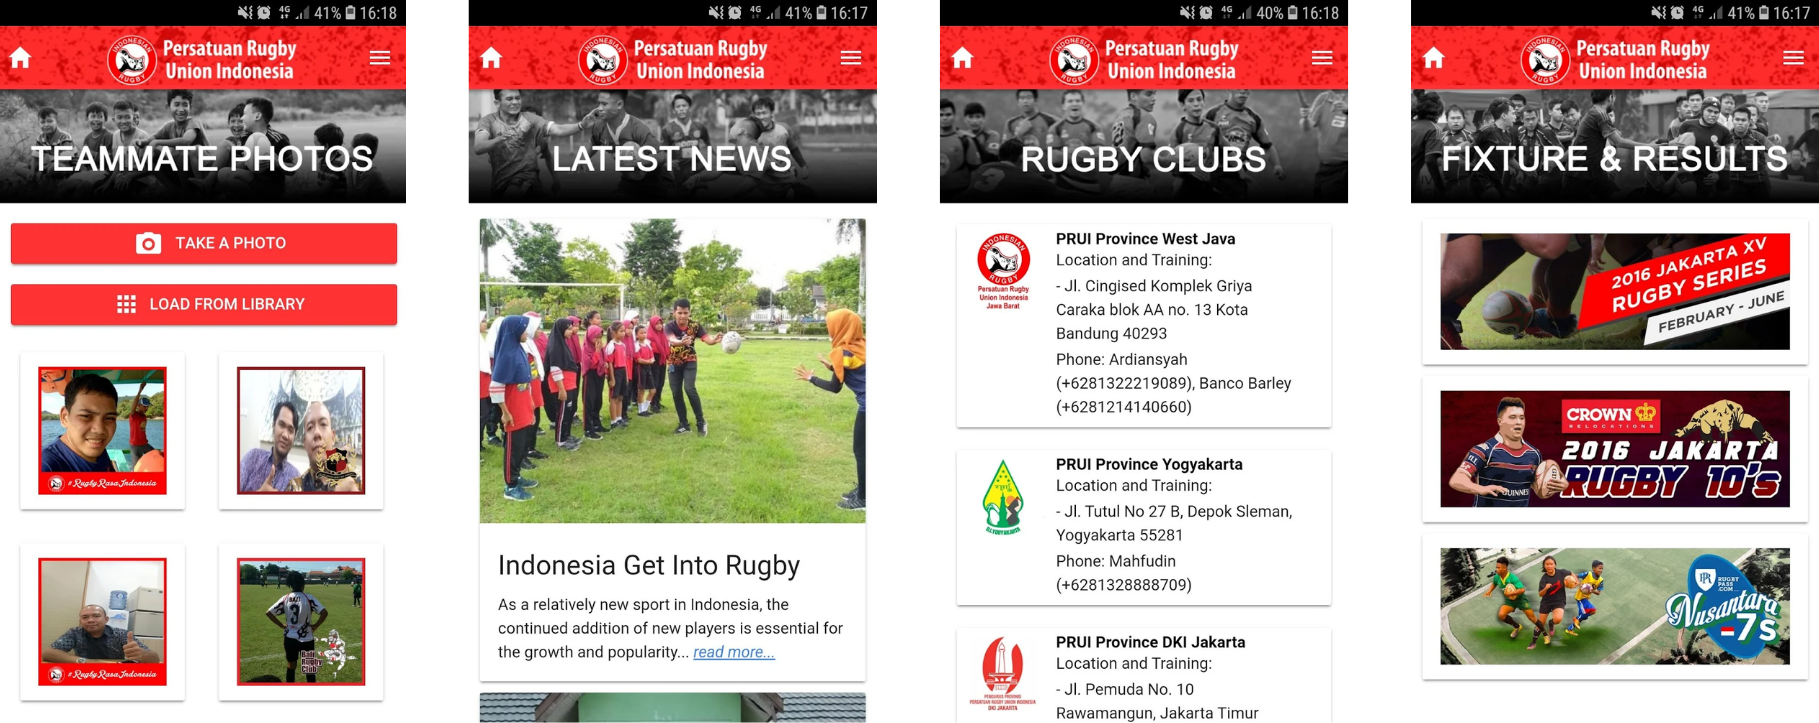
\includegraphics[scale=0.725]{Gambar/Rugby-Indonesia-App-UI.png}
    \caption[Halaman aplikasi Rugby Indonesia]{Halaman-halaman dari aplikasi Rugby Indonesia}
    \label{fig:rugby-halaman-label}
\end{figure}

Pada saat ini, aplikasi tersebut masih tersedia di Google Play Store\footnote{https://play.google.com/store/apps/details?id=id.or.rugbyindonesia.androidapp\&hl=in}, namun aplikasi tersebut tidak dapat dipasang pada perangkat android saat ini dikarenakan \textit{website} \url{https://rugbyindonesia.or.id} sudah berubah dan juga \textit{framework} yang digunakan sudah terlalu lama. Maka dari itu pada skripsi ini, akan dibuat ulang sebuah perangkat lunak Rugby Indonesia yang terbaru, sehingga perangkat lunak tersebut dapat \textit{compatible} dengan perangkat android saat ini.

Perangkat lunak ini akan dibuat dengan memanfaatkan bantuan {\it framework} Ionic 7 dan Capacitor dengan:

\begin{itemize}
    \item Halaman \textit{Latest News}, di mana pengguna dapat melihat berita terbaru seputar Rugby Indonesia.
    \item Halaman \textit{Teammate Photos}.
    \item Fitur lain yang akan ditambahkan ketika dibutuhkan.
\end{itemize}

% Bagian ini akan diisi dengan apa yang melatarbelakangi pembuatan template skripsi ini.
% Termasuk juga masalah-masalah yang akan dihadapi untuk membuatnya, termasuk kurangnya kemampuan penguasaan \LaTeX{} sehingga template ini dibuat dengan mengandalkan berbagai contoh yang tersebar di dunia maya, yang digabung-gabung menjadi satu jua.
% Bagian lain juga akan dilengkapi, untuk sementara diisi dengan lorem ipsum versi bahasa inggris.

% \dtext{5-10}

\section{Rumusan Masalah}
\label{sec:rumusan}
Rumusan masalah yang akan dibahas pada tugas akhir ini adalah sebagai berikut:
\begin{enumerate}
    \item Bagaimana cara membangun ulang serta mengembangkan perangkat lunak Rugby Indonesia dengan memanfaatkan \textit{framework} Ionic 7?
    \item Bagaimana cara menggunakan Capacitor pada pembangunan perangkat lunak Rugby Indonesia agar pengguna dapat mengunggah foto dengan mudah?
\end{enumerate}
% Bagian ini akan diisi dengan penajaman dari masalah-masalah yang sudah diidentifikasi di bagian sebelumnya. 

% \dtext{6}

\section{Tujuan}
\label{sec:tujuan}
Tujuan yang ingin dicapai pada penulisan tugas akhir ini yaitu:
\begin{enumerate}
    \item Dapat mengetahui bagaimana Ionic 7 memungkinkan pengembangan aplikasi Rugby Indonesia.
    \item Mengidentifikasi cara kerja dari Capacitor pada pembangunan perangkat lunak Rugby Indonesia.
\end{enumerate}
% Akan dipaparkan secara lebih terperinci dan tersturkur apa yang menjadi tujuan pembuatan template skripsi ini

% \dtext{7}

\section{Batasan Masalah}
\label{sec:batasan}
Batasan masalah yang terdapat pada pengerjaan tugas akhir ini yaitu:
\begin{itemize}
    \item Perangkat lunak ini memang sudah pernah dibuat pada tahun 2015 sebelumnya, namun perangkat lunak ini masih dibuat dengan menggunakan Apache Cordova, sehingga dokumentasi yang ada cukup berbeda dengan Ionic 7.
    \item Perangkat lunak ini hanya memfokuskan kepada aplikasi Rugby Indonesia saja.
    \item Pembuatan ulang perangkat lunak ini akan hanya mencakup fitur-fitur dasar seperti login, pengelolaan profil pengguna, dan pengambilan foto.
\end{itemize}
% Untuk mempermudah pembuatan template ini, tentu ada hal-hal yang harus dibatasi, misalnya saja bahwa template ini bukan berupa style \LaTeX{} pada umumnya (dengan alasannya karena belum mampu jika diminta membuat seperti itu)

% \dtext{8}

\section{Metodologi}
\label{sec:metlit}
% Tentunya akan diisi dengan metodologi yang serius sehingga templatenya terkesan lebih serius.

\dtext{9}

\section{Sistematika Pembahasan}
\label{sec:sispem}
% Rencananya Bab 2 akan berisi petunjuk penggunaan template dan dasar-dasar \LaTeX.
% Mungkin bab 3,4,5 dapt diisi oleh ketiga jurusan, misalnya peraturan dasar skripsi atau pedoman penulisan, tentu jika berkenan.
% Bab 6 akan diisi dengan kesimpulan, bahwa membuat template ini ternyata sungguh menghabiskan banyak waktu.

\dtext{10}